\section{2D Vision 1}\label{d-vision-1}

\subsection{Classification Backbones}\label{classification-backbones}

\subsubsection{Conceptions}\label{conceptions}

\textbf{Backbone}（主干网络）指用于提取图像通用特征的 CNN
模块，后续可以接负责具体任务（如分类）的 \textbf{head}。

从 ImageNet 的优胜模型演化我们可以看出 Backbone 的一些 implementation
details。 历史的顺序为 \textbf{AlexNet}、\textbf{VGG}、\textbf{ResNet}
等。

\textbf{Backbone 性能分析}：

\begin{itemize}
\tightlist
\item
  \textbf{Expressivity/Capacity}：模型能表示函数的复杂程度。
\item
  \textbf{Fitness for task}：对细粒度识别需要既有细节又有上下文。
\item
  \textbf{Optimization properties}：可训练性。
\item
  \textbf{Cost}：计算量、参数量、内存占用和推理延迟。
\end{itemize}

\centering
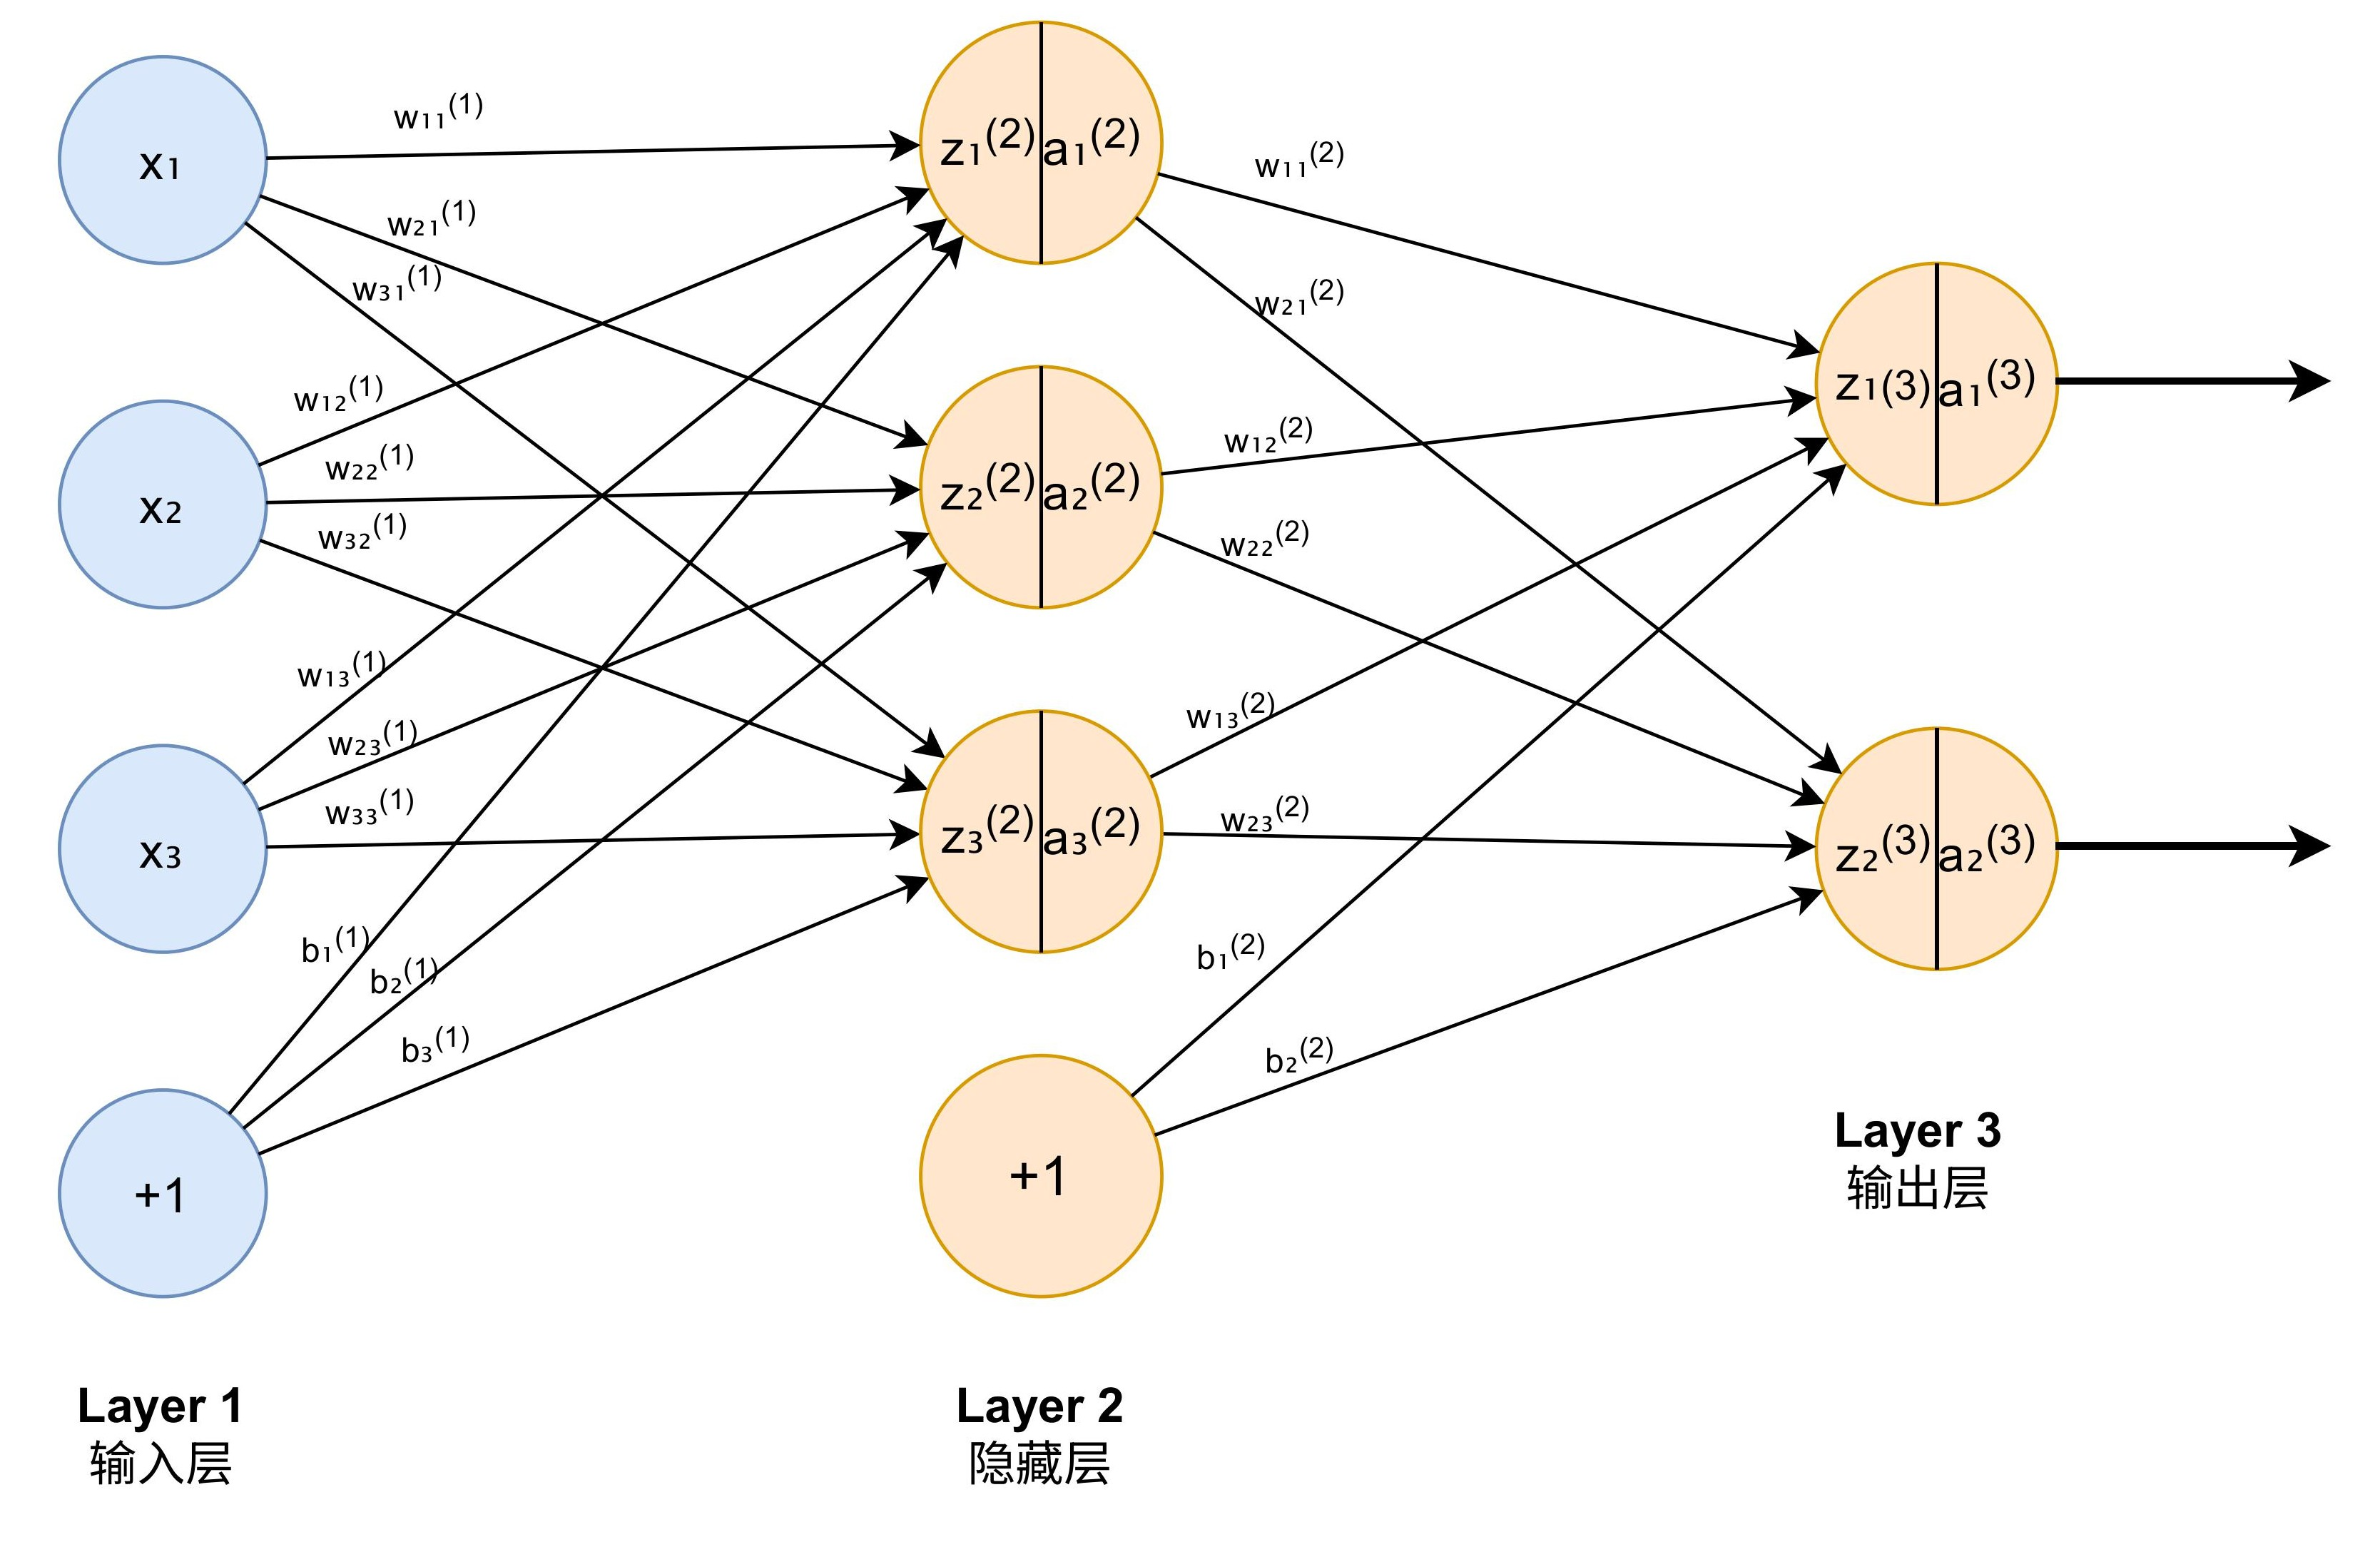
\includegraphics[width=\linewidth]{assets/07-2D-vision-1-01-neural-network.jpg}
\captionof{figure}{图 1：神经网络示意图，其中有竖线的橙色圆圈代表 neurons，有向边代表 params。neurons 对应了内存占用，params 对应了参数量}

\subsubsection{From AlexNet to VGG}\label{from-alexnet-to-vgg}

VGG 相比 AlexNet 使用了更深的层数和更小的 filter。

\textbf{感受野}：

网络中影响一个神经元输出的输入像素范围称为该神经元的 \textbf{Receptive
Field}（感受野）。

\textbf{感受野的递推公式}：

设第 \(\ell\) 层 kernel 大小为 \(k_{\ell}\)，stride 为
\(s_{\ell}\)，receptive field 为 \[f_{\ell}\]。 注意第 \(\ell\) 层的
kernel 作用于第 \(\ell\) 层的输入，输出第 \(\ell + 1\) 层的特征。

定义第 \(\ell\) 层的 jump 为 \(j_{\ell}\)，也即第 \(\ell\)
层相邻激活对应输入像素的间距。则： \[
\begin{aligned}
j_{\ell} &= s_{\ell-1} \cdot j_{\ell-1} = \prod_{i=1}^{\ell-1} s_i, \quad j_1 = 1 \\
f_{\ell} &= f_{\ell-1} + (k_{\ell-1} - 1) \cdot j_{\ell-1}, \quad f_1 = 1
\end{aligned}
\]

\textbf{证明}：

jump 的递推公式是显然的。

对于 receptive field，考虑第 \(\ell\) 层的一个神经元，它可以感受到第
\(\ell-1\) 层中跨度 \(k_{\ell-1}\) 个神经元。 它能感受到的第 \(\ell-1\)
层神经元的\textbf{所有感受野堆叠}形成的区域就是它自身的感受野。

这 \(k_{\ell-1}\)
个神经元各自的感受野在输入层上会有重叠，如下图所示。故重叠大小为： \[
\text{overlap} = f_{\ell-1} - j_{\ell-1}
\] 从而整体感受野长度为： \[
f_{\ell} = f_{\ell-1} + (k_{\ell-1}-1) \cdot j_{\ell-1}
\]

当然，这里面还需确保感受野确实是重叠的，或者说感受野之间\textbf{没有空隙}。也即验证：
\[
f_\ell \ge j_\ell
\] 代数化简得只需满足 \(k_\ell \ge s_\ell\)，上式即自动满足。

\centering
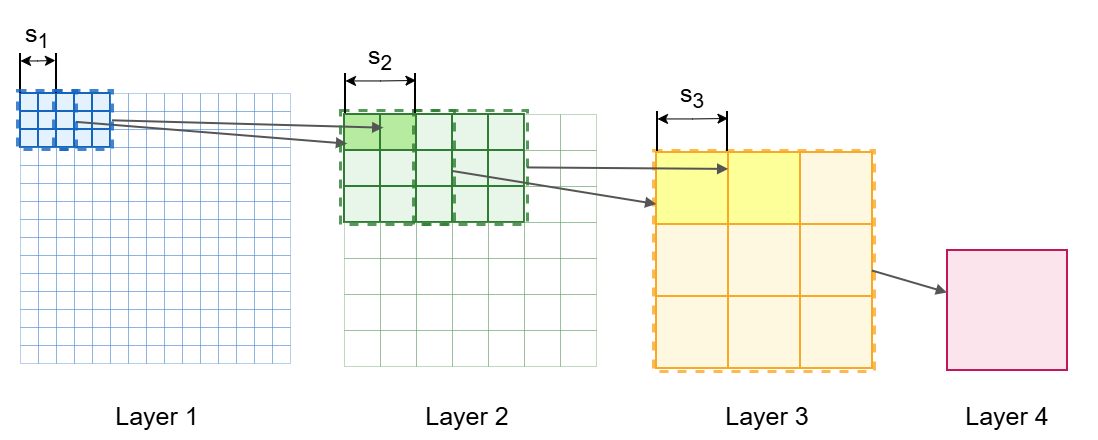
\includegraphics[width=\linewidth]{assets/07-2D-vision-1-02-receptive-field-1.png}
\captionof{figure}{图 2：感受野的递推公式 1，Conv 层示例，虚线框代表 kernel}

\centering
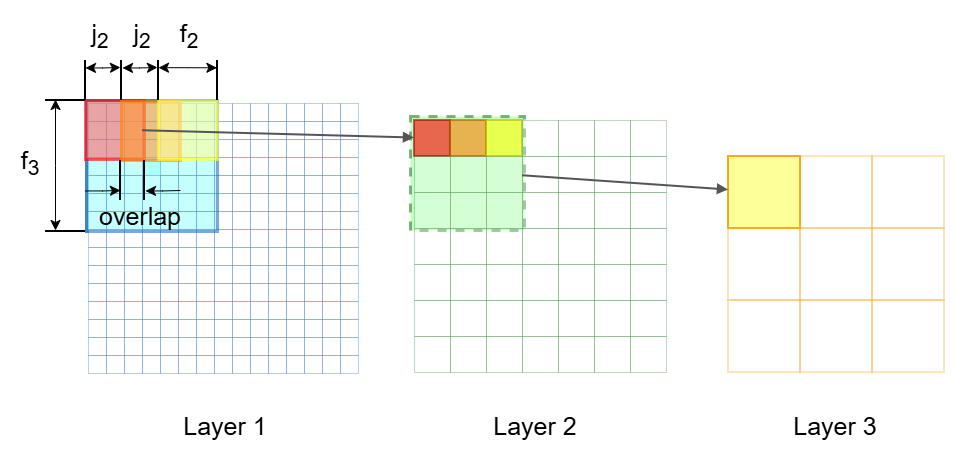
\includegraphics[width=\linewidth]{assets/07-2D-vision-1-03-receptive-field-2.png}
\captionof{figure}{图 3：感受野的递推公式 2，计算 $f_3$，实线框代表 field}

\centering
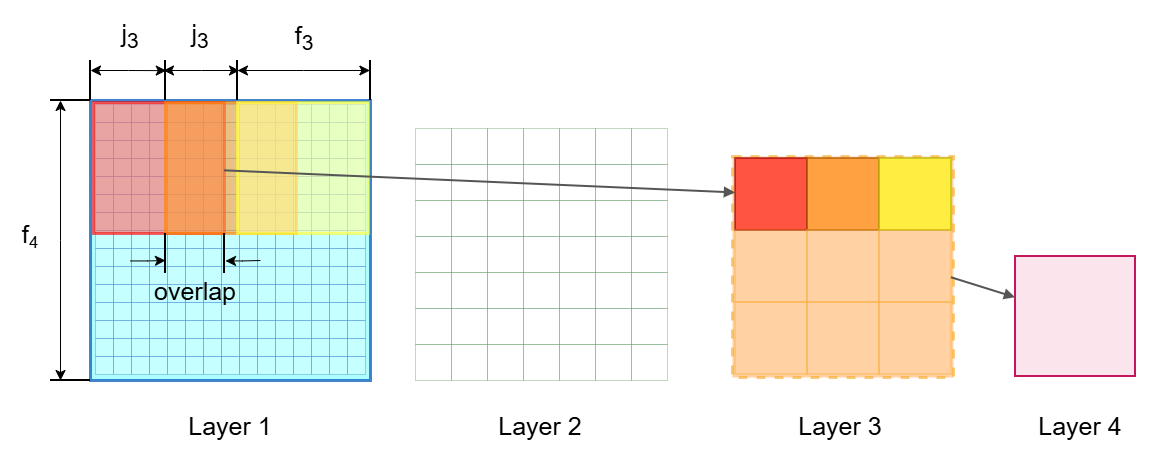
\includegraphics[width=\linewidth]{assets/07-2D-vision-1-04-receptive-field-3.png}
\captionof{figure}{图 4：感受野的递推公式 3，计算 $f_4$，实线框代表 field}

\textbf{smaller kernel \& deeper net 的好处}：

\begin{itemize}
\tightlist
\item
  多层小 filter 与单层大 filter 可以获得\textbf{相同的感受野}。
\item
  层数越多，激活越多，\textbf{nonlinear} 越强，capacity 越强。
\item
  参数更少。
\end{itemize}

举例来说，取 stride 均为 \(1\)，且输入输出通道始终为 \(C\)。

则 \(3\) 层 \(3 \times 3\) Conv 与 \(1\) 层 \(7 \times 7\) Conv
感受野相同。

但是前者有 \(3\) 次激活，只需 \(3 \cdot (3^2 C^2)\) 参数； 后者只有
\(1\) 次激活，需要 \(7^2 C^2\) 参数。

\textbf{注}：
感受野不是越大越好。太大可能带来过多噪声，而太小则无法捕获全局上下文。

\subsubsection{From VGG to ResNet}\label{from-vgg-to-resnet}

ResNet 相比 VGG 网络深度有了显著的提升，主要是因为使用了
\textbf{Residual Block}。 有关内容见前述笔记
Residual Link。

同时 ResNet 还引入了 \textbf{bottleneck}（瓶颈层）。 Bottleneck
的核心是先提炼关键信息，只在关键信息上做昂贵的大卷积核运算，从而\textbf{减少参数量}。

具体来说：

\begin{itemize}
\tightlist
\item
  先用 \(64\) 个 \(1 \times 1\) 的 kernel 把 \(256\) 维特征压缩到 \(64\)
  维子空间。
\item
  然后用 \(64\) 个 \(3 \times 3\) 的 kernel 进行空间特征提取，
\item
  最后再用 \(256\) 个 \(1 \times 1\) 的 kernel 升维回 \(256\) 维。
\end{itemize}

下图中两种 block 均完成了 \(28 \times 28 \times 256\) 到
\(28 \times 28 \times 256\) 的映射，对比两者的参数量：

\begin{itemize}
\tightlist
\item
  Basic Block：\(2 (3^2 \times 256^2) \approx 1.18 \text{M}\)
\item
  Bottleneck：\(1^2 \times 256 \times 64 + 3^2 \times 64^2 + 1^2 \times 64 \times 256 \approx 70 \text{K}\)
\end{itemize}

\centering
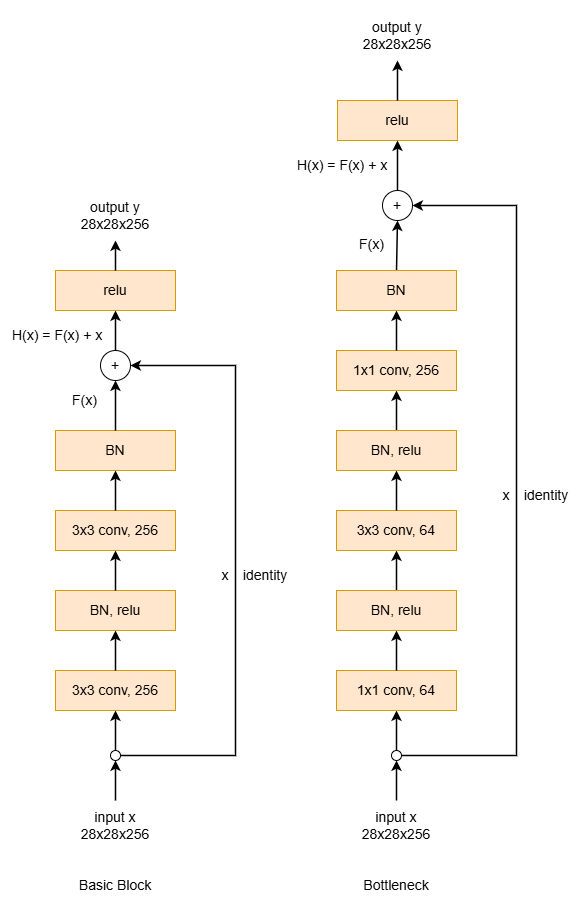
\includegraphics[width=\linewidth]{assets/07-2D-vision-1-05-bottleneck.png}
\captionof{figure}{图 5：Bottleneck}

\subsubsection{Beyond ResNet}\label{beyond-resnet}

ResNet 对于 CNN 的开发已基本完善。不过后续还有诸多变体。

\begin{itemize}
\item
  \textbf{SENet}：通道注意力，通过学习通道权重来加强重要通道的特征。
\item
  \textbf{DenseNet}：密集连接，每层接收前面所有层的特征并 concatenate
  为后续输入。
\item
  \textbf{MobileNet}：深度可分离卷积（\textbf{Depthwise Separable
  Convolution}），将标准卷积拆分为两步，降低计算成本，使 CNN
  可在移动端实时运行。
  本质上是把对\textbf{空间的混合}和对\textbf{通道的混合}解耦开了。

  \begin{itemize}
  \item
    \textbf{标准卷积（图 a）}：\\
    对于 \(H \times W \times M\) 的输入，要得到 \(N\)
    个输出通道，每个输出通道需要一组卷积核。 每组包含 \(M\) 个
    \(D_k \times D_k\) 的 kernel，分别对应 \(M\)
    个输入通道；卷积结果在通道维度上求和，得到一个输出通道。因此总共需要
    \(N\) 组。

    计算量为 \(D_k^2 \cdot M \cdot N \cdot H \cdot W\)。
  \item
    \textbf{MobileNet（图 b-c）}：\\
    将上述过程解耦为两步。

    \begin{enumerate}
    \def\labelenumi{\arabic{enumi}.}
    \item
      \textbf{Depthwise 卷积（图 b）}：\\
      对 \(H \times W \times M\)
      的输入，每个输入通道单独做\textbf{空间卷积}。 每个通道只用 \(1\)
      个 \(D_k \times D_k\) 的 kernel，共需 \(M\) 个 kernel。
      此时输出仍为 \(H \times W \times M\)。

      计算量为 \(D_k^2 \cdot M \cdot H \cdot W\)。
    \item
      \textbf{Pointwise 卷积（图 c）}：\\
      使用 \(1 \times 1\) 卷积将 \(M\) 个\textbf{通道混合}为 \(N\)
      个输出通道。 每个输出通道需要 \(M\) 个 \(1 \times 1\) 的
      kernel，共需 \(N\) 组。

      计算量为 \(1^2 \cdot M \cdot N \cdot H \cdot W\)。
    \end{enumerate}

    当通道数 \(N\) 较大时，计算量约为标准卷积的
    \(1/N\)，精度损失却很小。
  \end{itemize}
\end{itemize}

\centering
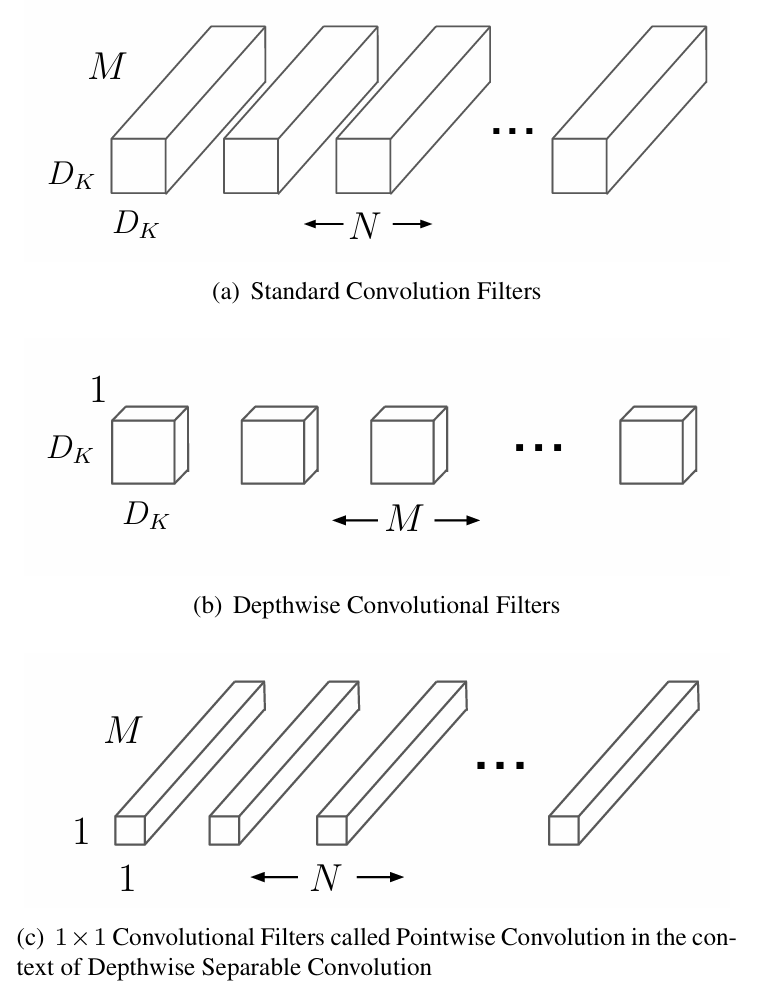
\includegraphics[width=\linewidth]{assets/07-2D-vision-1-06-mobilenet.png}
\captionof{figure}{图 6：深度可分离卷积}

\begin{itemize}
\tightlist
\item
  \textbf{NAS}（Neural Architecture
  Search）：使用学习算法自动搜索网络结构。
\end{itemize}

\begin{center}\rule{0.5\linewidth}{0.5pt}\end{center}

\subsection{Segmentation}\label{segmentation}

\subsubsection{Defination}\label{defination}

图像分割是将图像中属于不同语义/实例的像素分组的任务。也即
\textbf{Pixel-based Classification}。

\begin{itemize}
\tightlist
\item
  \textbf{Semantic
  Segmentation}：语义分割，逐像素预测类别，不区分同类不同实例。
\item
  \textbf{Instance
  Segmentation}：实例分割，逐像素预测类别，且区分同类不同实例。
\item
  \textbf{Semantic Instance
  Segmentation}：前两者的结合，对前景物体（things）进行实例分割，对背景（stuff）只进行语义分类。
\end{itemize}

\subsubsection{FCN}\label{fcn}

全卷积网络（Fully Convolution
Network）可以接受任意输入尺寸，并输出与输入同尺寸的预测图。

但是图像尺寸实在是太大了，我们需要使用 \textbf{Bottleneck}
思想，采用以下 \textbf{Auto-Encoder} 框架：

\begin{itemize}
\item
  \textbf{Encoder}： 执行
  downsampling，内存占用和参数量更小，感受野更大。

  设输入图像为
  \(x\in\mathbb{R}^{C_0\times H_0\times W_0}\)，下采样模块共 \(L\)
  层，\(s_\ell\) 为第 \(\ell\) 层的下采样因子（如 Conv 的 stride）。
  则总下采样因子为： \[
    D=\prod_{\ell=1}^L s_\ell
    \] 从而得到瓶颈处的空间尺寸： \[
    H_L=\left\lfloor\frac{H_0}{D}\right\rfloor,\quad
    W_L=\left\lfloor\frac{W_0}{D}\right\rfloor
    \] 整个 Encoder 可视为一个参数化映射 \(E_\theta\)，参数集合为
  \(\theta\)，满足： \[
    E_\theta:\; \mathcal{X}\to\mathcal{Z},\qquad
    x\mapsto Z=E_\theta(x)\in\mathbb{R}^{C_L\times H_L\times W_L}
    \] 其中 \(C_L\) 为瓶颈处通道数。
\item
  \textbf{Decoder}： 执行 upsampling，将瓶颈特征恢复至原始尺寸。

  设上采样模块共 \(L'\) 层，第 \(k\) 层的上采样因子（如 ConvTranspose 的
  stride）为 \(t_k\)。 则总上采样因子为： \[
    U = \prod_{k=1}^{L'} t_k
    \] 为保证输出尺寸与输入一致，通常有 \(U = D\)，且： \[
    H_0 \approx U \cdot H_L,\quad
    W_0 \approx U \cdot W_L
    \]

  整个 Decoder 可视为一个参数化映射 \(D_\phi\)，参数集合为 \(\phi\)。

  当用于图像重构时，记为： \[
    D_\phi:\; \mathcal{Z} \to \hat{\mathcal{X}},\qquad
    Z \mapsto \hat{x} = D_\phi(Z) \in \mathbb{R}^{C_0 \times H_0 \times W_0}
    \] 其中 \(\hat{x} = D_\phi(E_\theta(x))\) 为重构输出，\(C_0\)
  为输出通道数（如 RGB 图像为 3）。

  当用于语义分割时，记为： \[
    D_\phi:\; \mathcal{Z} \to \hat{\mathcal{Y}},\qquad
    Z \mapsto \hat{y} = D_\phi(Z) \in \mathbb{R}^{K \times H_0 \times W_0}
    \] 其中 \(K\) 为类别数，\(\hat{y}_{c,i,j}\) 表示位置 \((i,j)\)
  属于类别 \(c\) 的预测概率。
\item
  \textbf{Loss Function}： 取决于具体的任务。

  对于图像重构： \[
    \mathcal{L}_{\text{rebuild}}(\theta,\phi)
    = \mathbb{E}_{x \sim p_{\text{data}}}\left[ \| x - \hat{x} \|_2^2 \right]
    \] 对于语义分割： \[
    \mathcal{L}_{\text{seg}}(\theta,\phi)
    = -\frac{1}{H_0 W_0} \sum_{i=1}^{H_0} \sum_{j=1}^{W_0} \sum_{c=1}^{K} y_{c,i,j} \log \hat{y}_{c,i,j}
    \] 其中 \(y_{c,i,j} \in \{0,1\}\) 为位置 \((i,j)\) 的 one-hot
  真实标签，\(\hat{y}_{c,i,j} \in [0,1]\) 为模型预测概率。
\end{itemize}

\textbf{Bottleneck Pros}：

\begin{itemize}
\tightlist
\item
  内存占用更低，对于高分辨率图像来说很重要。
\item
  在更小特征图上进行 conv，等效感受野更大，能以更低 cost 捕获更大范围
  context。
\end{itemize}

\textbf{注}：
本质上日常生活中的图像都是内嵌于高维空间的低维流形（minifold）。
通过压缩可以保留重要语义，丢弃冗余信息，便于进一步语义分割。

\subsubsection{Non-learnable Upsampling}\label{non-learnable-upsampling}

\begin{enumerate}
\def\labelenumi{\arabic{enumi}.}
\tightlist
\item
  \textbf{Bilinear}：双线性插值。目标像素在源图像中计算坐标，然后做插值。
\item
  \textbf{Nearest Neighbor Unpooling}：最近邻上采样。将每个像素放大为
  \(r \times r\) 的 block，block 内都填充像素值，其中 \(r\)
  为上采样因子。
\item
  \textbf{Bed of Nails Unpooling}：零填充上采样。将每个像素放大为
  \(r \times r\) 的 block，block 左上角填充像素值，其余为 \(0\)，其中
  \(r\) 为上采样因子。
\item
  \textbf{Max Unpooling}：与 \textbf{Max Pooling} 配对使用。
  Downsampling 时记录每个 pooling window 中最大值的位置索引； Upsampling
  时，将每个输入值放回原来的位置，其余位置置 \(0\)。
\end{enumerate}


\centering
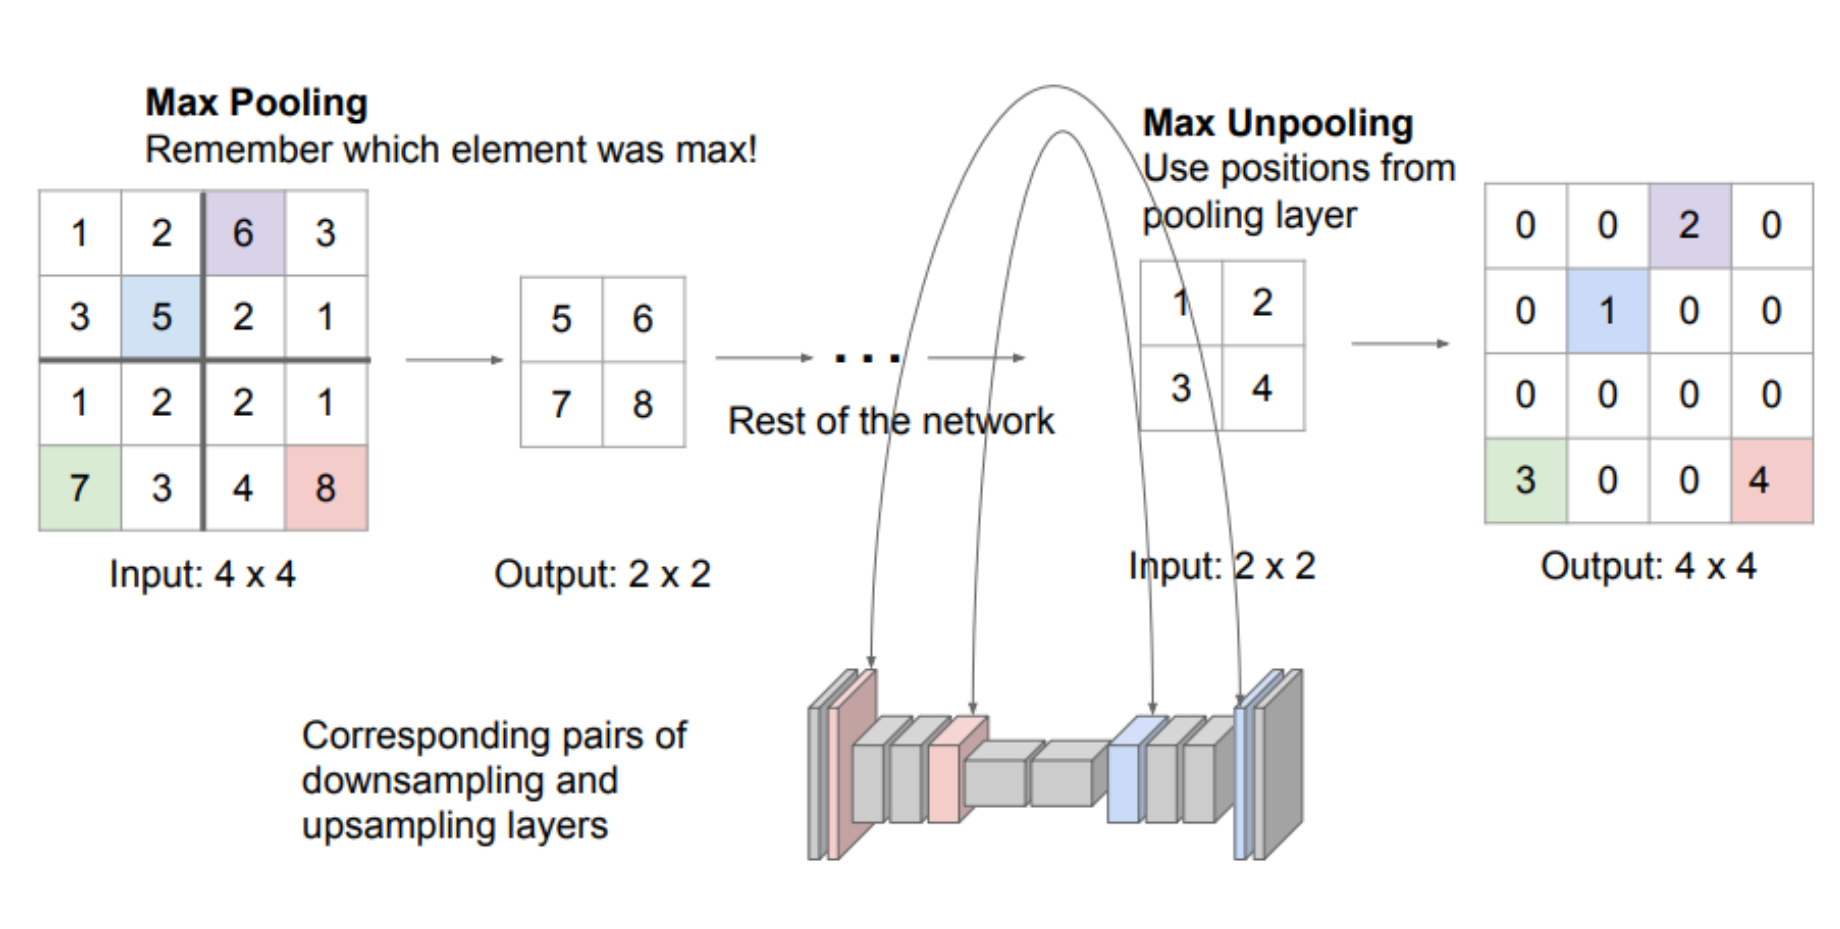
\includegraphics[width=\linewidth]{assets/07-2D-vision-1-07-max-unpooling.png}
\captionof{figure}{图 7：Max Unpooling}

\subsubsection{Learnable Upsampling}\label{learnable-upsampling}

\textbf{Transposed Convolution}（转置卷积）。

部分文献中也称为 \emph{Deconvolution}（反卷积），但数学上的
deconvolution
定义为卷积的逆运算，而转置卷积\textbf{并不保证恢复原始输入}，因此并不合适。

\textbf{定义}：

普通卷积可展开为稀疏的 Toeplitz 矩阵 \(\mathbf{C}\)，使得

\[
y = w * x = \mathbf{C}x
\]

转置卷积即在该矩阵表示下，使用 \(\mathbf{C}^\top\) 进行乘法：

\[
x = w *^\top y = \mathbf{C}^\top y
\]

由于普通卷积的反向传播时有： \[
\frac{\partial \mathcal{L}}{\partial x} = \mathbf{C}^\top \frac{\partial \mathcal{L}}{\partial y}
\]

\textbf{转置卷积的前向传播}恰好对应上述 \(\mathbf{C}^\top\)
的乘法操作。因此它常被描述为普通卷积在 backpropagation 时的梯度运算。

\textbf{等价性}：

转置卷积可以用\textbf{普通卷积}来模拟。

考虑一个普通卷积：

\begin{itemize}
\tightlist
\item
  输入尺寸为 \(h_{in} \times w_{in}\)
\item
  参数为 kernel \(k\)、stride \(s\)、padding \(p\)
\item
  输出尺寸为 \(h_{out} \times w_{out}\)
\end{itemize}

与之对应的转置卷积与之\textbf{共享同一组参数}
\((k, s, p)\)，且尺寸满足： \[
\begin{aligned}
h_{in}' = h_{out},& \quad h_{out}' = h_{in} \\
w_{in}' = w_{out},& \quad w_{out}' = w_{in}
\end{aligned}
\]

概念上，该转置卷积等价于对输入 \(h_{in}' \times w_{in}'\)
执行以下普通卷积：

\begin{enumerate}
\def\labelenumi{\arabic{enumi}.}
\tightlist
\item
  \textbf{Stretching}：在输入像素之间插入 \(s-1\) 个零；
\item
  \textbf{Surrounding padding}：四周填充 \(k - p - 1\) 个零；
\item
  \textbf{Additional padding}：若 \(h_{in} + 2p - k\) 不能被 \(s\)
  整除，还需在输入的 bottom 和 right 额外补 \(a\) 个零，其中 \[
   a = \bigl(h_{in} + 2p - k\bigr) \bmod s, \quad a \in \{0, 1, \dots, s-1\}
   \] 这里 \(h_{in}\) 即转置卷积期望的输出尺寸 \(h_{out}'\)；
\item
  \textbf{Convolution}：使用 unit stride \(s' = 1\) 和 kernel \(k\)
  进行卷积。
\end{enumerate}

转置卷积的输出尺寸公式为： \[
\begin{aligned}
h_{out}' &= s\bigl(h_{in}' - 1\bigr) + a + k - 2p \\
w_{out}' &= s\bigl(w_{in}' - 1\bigr) + a + k - 2p
\end{aligned}
\]

下面是一些图示：

\begin{itemize}
\tightlist
\item
  图中下方蓝色的是执行了 Stretching、Surrounding padding 和 Additional
  padding 后的图像。
\item
  图中上方是使用等价 convolution 后，也即 Transposed Convolution
  后得到的上采样图像。
\end{itemize}

% \centering
% \includegraphics[width=\linewidth]{assets/07-2D-vision-1-08-no-padding-no-stride-transposed.gif}
% \captionof{figure}{图 8：$h'_{\text{in}}=2$, $h'_{\text{out}}=4$, $k=3$, $s=1$, $p=0$}

% \centering
% \includegraphics[width=\linewidth]{assets/07-2D-vision-1-09-same-padding-no-stride-transposed.gif}
% \captionof{figure}{图 9：same padding, $h'_{\text{in}}=5$, $h'_{\text{out}}=5$, $k=3$, $s=1$, $p=(k-1)/2$}

% \centering
% \includegraphics[width=\linewidth]{assets/07-2D-vision-1-10-full-padding-no-stride-transposed.gif}
% \captionof{figure}{图 10：full padding, $h'_{\text{in}}=7$, $h'_{\text{out}}=5$, $k=3$, $s=1$, $p=k-1$}

% \centering
% \includegraphics[width=\linewidth]{assets/07-2D-vision-1-11-no-padding-with-stride-transposed.gif}
% \captionof{figure}{图 11：$h'_{\text{in}}=2$, $h'_{\text{out}}=5$, $k=3$, $s=2$, $p=0$}

% \centering
% \includegraphics[width=\linewidth]{assets/07-2D-vision-1-12-with-padding-with-stride-transposed.gif}
% \captionof{figure}{图 12：$h'_{\text{in}}=3$, $h'_{\text{out}}=5$, $k=3$, $s=2$, $p=1$}

% \centering
% \includegraphics[width=\linewidth]{assets/07-2D-vision-1-13-with-padding-with-strides-with-addition-transposed.gif}
% \captionof{figure}{图 13：$h'_{\text{in}}=3$, $h'_{\text{out}}=6$, $k=3$, $s=2$, $p=1$}

\textbf{注}：这只是\textbf{概念上等价}的示意方法。实际软件实现不会真的插入大量零再做乘法，因为那样会产生大量无效的零乘运算，效率极低。

\textbf{Checkerboard Artifacts}：

转置卷积的一个已知缺陷是：当 kernel 尺寸 \(k\) 不能被 stride \(s\)
整除时，kernel
在输出空间上的重叠区域不均匀，导致叠加后累积激活强度不一致，产生周期性的\textbf{棋盘格伪影}。

\centering
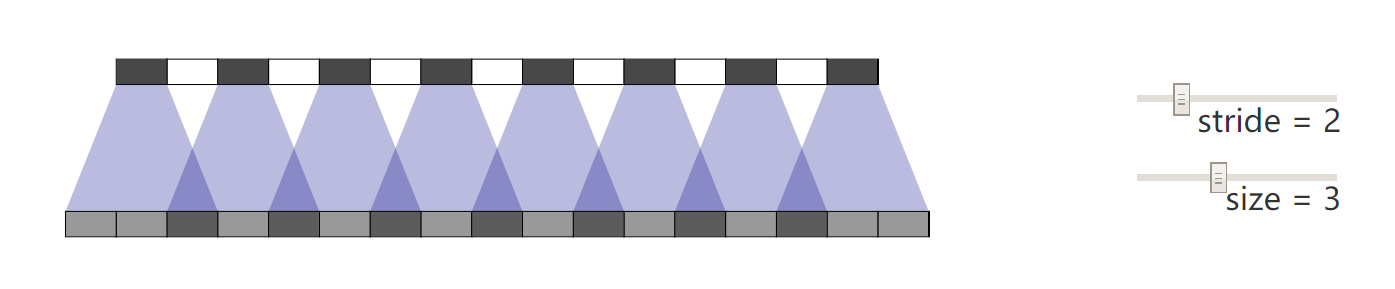
\includegraphics[width=\linewidth]{assets/07-2D-vision-1-14-1d-checkerboard-artifacts.png}
\captionof{figure}{图 14：一维棋盘格伪影}

\centering
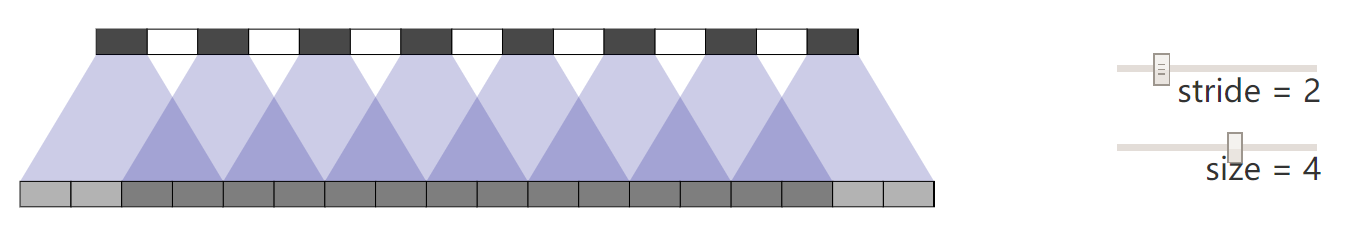
\includegraphics[width=\linewidth]{assets/07-2D-vision-1-15-1d-no-checkerboard-artifacts.png}
\captionof{figure}{图 15：stride 整除 kernel 时没有伪影}

\centering
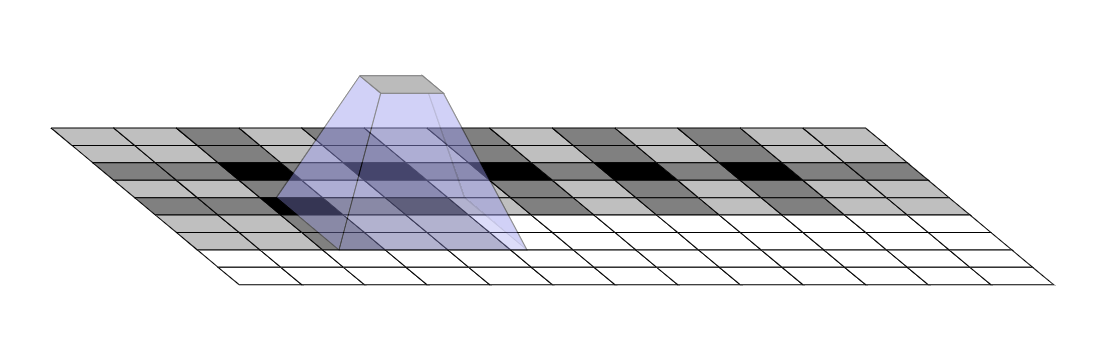
\includegraphics[width=\linewidth]{assets/07-2D-vision-1-16-2d-checkerboard-artifacts.png}
\captionof{figure}{图 16：二维棋盘格伪影}

\textbf{替代方案}：

\begin{itemize}
\tightlist
\item
  \textbf{PixelShuffle} / \textbf{Sub-pixel
  Convolution}：用一些神秘的手段天然避免了棋盘格问题。
\item
  \textbf{Resize-Conv}：先使用非学习型插值进行上采样，再用普通
  \(3\times3\) 卷积微调。
\end{itemize}

\subsubsection{UNet}\label{unet}

Network Architecture Design 的两个核心：

\begin{enumerate}
\def\labelenumi{\arabic{enumi}.}
\tightlist
\item
  \textbf{Information Sufficiency}：是否具备支持任务完成的充足信息。
  例如，分类任务需要足够大的感受野覆盖目标整体；分割任务则要求保留逐像素的空间定位信息。
\item
  \textbf{Optimization Feasibility}：是否利于优化。
  通常任务越复杂，网络的 capacity 要求越高，收敛难度也随之增大。
\end{enumerate}

FCN 的问题在于信息流单向串行，所以 Bottleneck
处必须同时承载\textbf{global context}与\textbf{per-pixel
spatial}，这使得 Bottleneck 承担了过度复杂的任务，优化困难。

UNet 在 Auto-Encoder 框架中加入 \textbf{Skip Link}，把 Encoder
中对应分辨率的特征直接拼接到 Decoder 的\textbf{对应层}。

从而 Bottleneck 只需负责 global context，Skip Link 补充 per-pixel
spatial，减轻了 Bottleneck 的负担。

注意此处的 Skip Link 执行的是 \textbf{Concatenation} 而非 Addition。

\centering
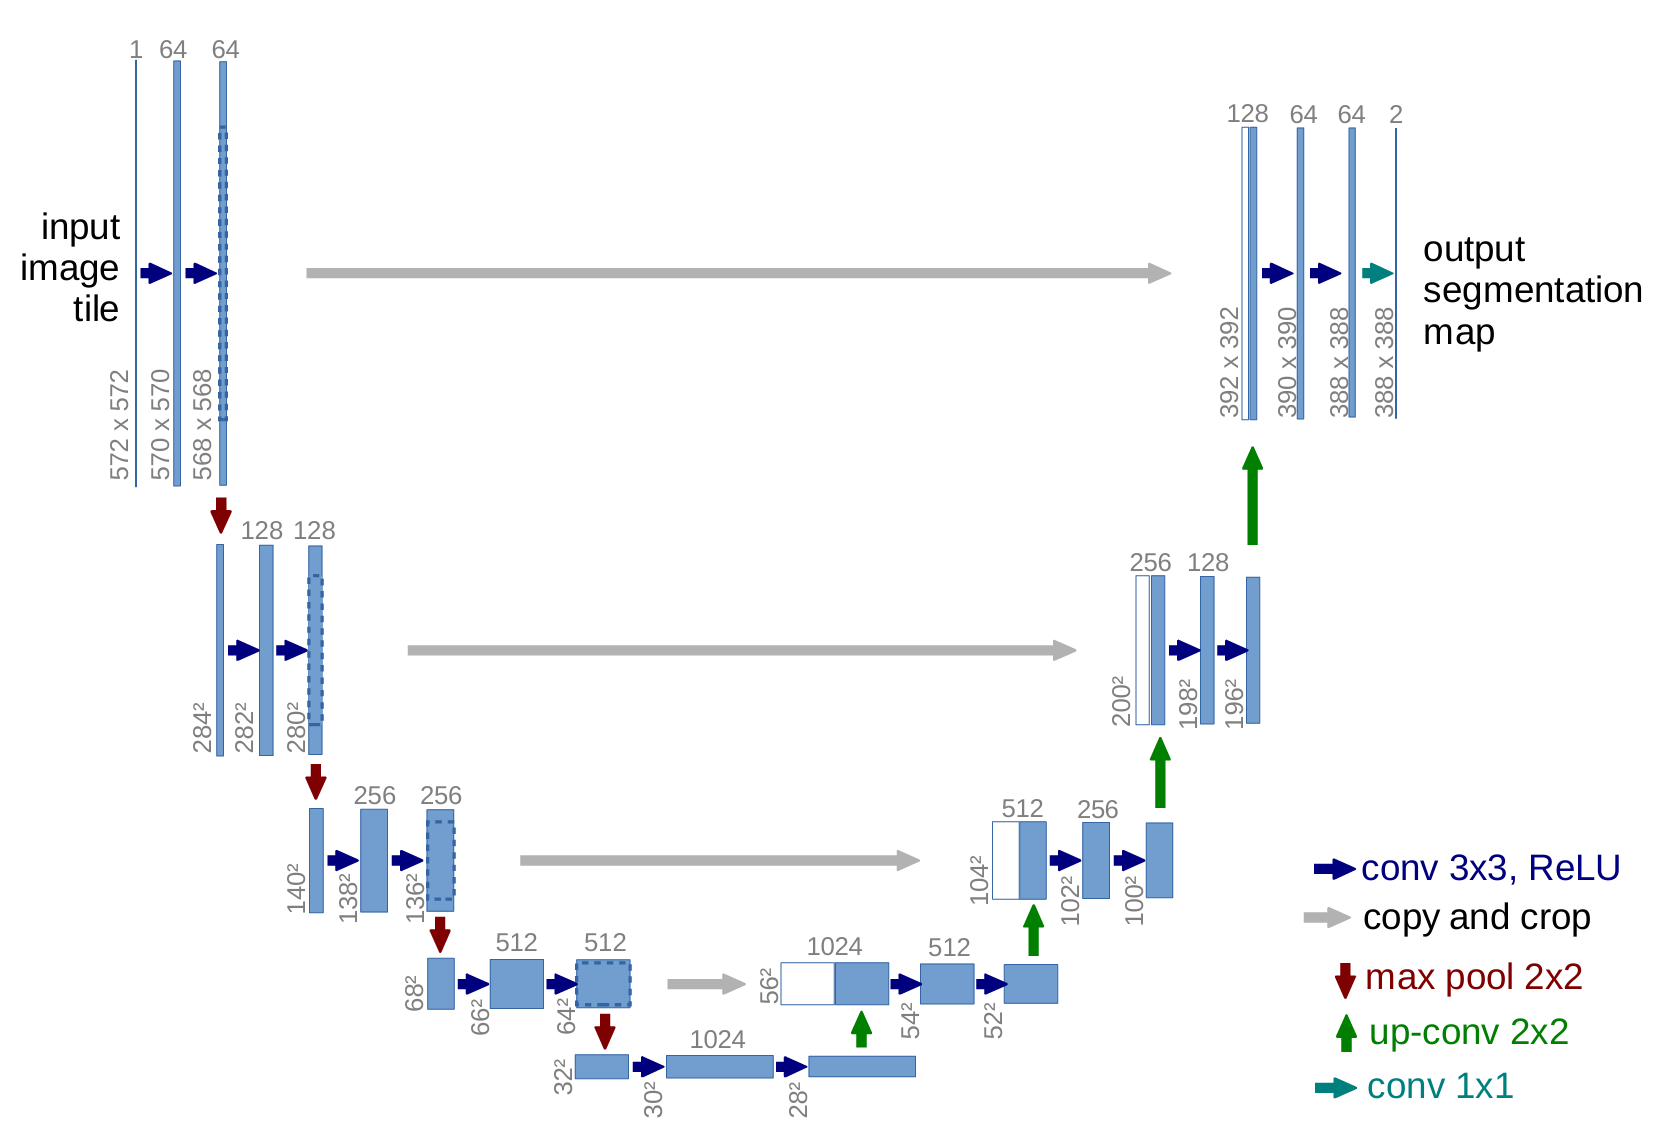
\includegraphics[width=\linewidth]{assets/07-2D-vision-1-17-UNet.png}
\captionof{figure}{图 17：UNet 架构}

\subsubsection{Evaluation Metrics}\label{evaluation-metrics}

\textbf{Pixel Accuracy}： \[
\text{Accuracy} = \dfrac{\text{TP}+\text{TN}}{\text{TP}+\text{TN}+\text{FP}+\text{FN}}
\] 问题在于当 positive 类占比极小时，准确率由 \(\text{TN}\)
主导，此时模型即使完全不预测 positive 类也有接近 100\% 的准确率。

\textbf{IoU}： Intersection over
Union，交并比，可用于评估某一类的分割能力。 \[
\text{IoU} = \frac{ | \text{Prediction} \cap \text{GroundTruth} | }{ | \text{Prediction} \cup \text{GroundTruth} | }
\] 其中 \(\text{Prediction}\) 为预测掩码，\(\text{GroundTruth}\)
为真值掩码。 二分类问题中即为： \[
\text{IoU} = \frac{\text{TP}}{\text{TP} + \text{FP} + \text{FN}}
\]

\textbf{注}：本质上只要是两个集合，就可以用 IoU 计算相似度。

\textbf{mIoU}： mean IoU
可用于评估对多类的整体分隔能力，也即对每个类计算 IoU，再取平均。 \[
\text{mIoU} = \frac{1}{K} \sum_{k=1}^{K} \text{IoU}_k
\] 其中 \(K\) 为总类数。

\textbf{注}： 对类别不平衡问题，mIoU 能公平考虑每个类的分割性能；

\subsubsection{Soft IoU Loss}\label{soft-iou-loss}

本质上 train objection 为 Loss function，而 test objection 为 Evaluation
metrics，两者往往不一致：

\begin{itemize}
\tightlist
\item
  \textbf{Loss Function}：作为训练目标，必须可导
\item
  \textbf{Evaluation Metrics}：真实任务需求，可能不可导
\end{itemize}

我们希望构造合适的 Loss function 以对齐 Evaluation metrics，从而缩小
surrogate gap。

\textbf{Soft IoU Loss}：

标准 IoU 基于离散的二值掩码，不可导。Soft IoU Loss 将其连续化。

设网络经 Sigmoid 或 Softmax 输出的概率图为 \(p\)，对应 one-hot 标签为
\(y\)。定义\textbf{软交集}与\textbf{软并集}：

\[
\begin{aligned}
\text{Soft Intersection} &= \sum_i p_i y_i \\
\text{Soft Union} &= 1 - \sum_i (1 - p_i)\cdot(1 - y_i) = \sum_i (p_i + y_i - p_i y_i)
\end{aligned}
\]

则 Soft IoU 为： \[
\text{Soft IoU}
= \frac{\text{Soft Intersection}}{Soft Union}
= \frac{\sum_i p_i y_i}{\sum_i p_i + \sum_i y_i - \sum_i p_i y_i}
\]

实现中通常加入平滑项 \(\epsilon\) 防止除零，并取 \(1 - \text{Soft IoU}\)
作为 Loss： \[
\mathcal{L}_{\text{IoU}} = 1 - \frac{\sum_i p_i y_i + \epsilon}{\sum_i p_i + \sum_i y_i - \sum_i p_i y_i + \epsilon}
\]

对于多类分割，可逐类取均值计算 mIoU Loss： \[
\mathcal{L}_{\text{mIoU}}
= 1 - \frac{1}{K} \sum_{k=1}^{K}
\frac{\sum_i p_{k,i} y_{k,i} + \epsilon}{\sum_i p_{k,i} + \sum_i y_{k,i} - \sum_i p_{k,i} y_{k,i} + \epsilon}
\]
